\documentclass[a4paper,landscape,8pt]{extarticle}
\usepackage[ngerman]{babel}
\usepackage{amsmath,amsthm}
\usepackage{ascii}
\usepackage[adobe-utopia]{mathdesign}
\usepackage[T1]{fontenc}
\usepackage[margin=0.5cm]{geometry}
\usepackage{multicol}
\usepackage{color,graphicx,overpic}
\usepackage{hyperref}
\newcommand{\ra}[1]{\renewcommand{\arraystretch}{#1}}
%Style imports
\usepackage[inline]{enumitem}
\usepackage{tcolorbox}
\usepackage{listings}
\usepackage{algorithm}
\usepackage{algpseudocode}
\usepackage{authblk}
\usepackage{fancyhdr}
\usepackage{fancyhdr}
\usepackage{datetime}
\usepackage[iso,german]{isodate}
%Graphic imports
\usepackage{tikz}
\graphicspath{ {./img/} }

% Turn off header and footer
\pagestyle{empty}

% Redefine section commands to use less space
\makeatletter
\renewcommand{\section}{\@startsection{section}{1}{0mm}%
                                {-1ex plus -.5ex minus -.2ex}%
                                {0.5ex plus .2ex}%x
                                {\normalfont\large\bfseries}}
\renewcommand{\subsection}{\@startsection{subsection}{2}{0mm}%
                                {-1explus -.5ex minus -.2ex}%
                                {0.5ex plus .2ex}%
                                {\normalfont\normalsize\bfseries}}
\renewcommand{\subsubsection}{\@startsection{subsubsection}{3}{0mm}%
                                {-1ex plus -.5ex minus -.2ex}%
                                {1ex plus .2ex}%
                                {\normalfont\small\bfseries}}
\renewcommand{\paragraph}{%
  \@startsection{paragraph}{4}%
  {\z@}{1ex \@plus 1ex \@minus .2ex}{-1em}%
  {\normalfont\normalsize\bfseries}%
}
\makeatother

% Define BibTeX command
\def\BibTeX{{\rm B\kern-.05em{\sc i\kern-.025em b}\kern-.08em
    T\kern-.1667em\lower.7ex\hbox{E}\kern-.125emX}}

% Don't print section numbers
\setcounter{secnumdepth}{0}

\setlength{\parindent}{0pt}
\setlength{\parskip}{0pt plus 0.5ex}

%My Environments
\newtheorem{example}[section]{Example}
% -----------------------------------------------------------------------
\definecolor{codegreen}{rgb}{0,0.6,0}
\definecolor{codegray}{rgb}{0.5,0.5,0.5}
\definecolor{codepurple}{rgb}{0.58,0,0.82}
\definecolor{backcolour}{rgb}{0.95,0.95,0.92}
\lstdefinelanguage{CSS}{
  morekeywords={accelerator,azimuth,background,background-attachment,
    background-color,background-image,background-position,
    background-position-x,background-position-y,background-repeat,
    behavior,border,border-bottom,border-bottom-color,
    border-bottom-style,border-bottom-width,border-collapse,
    border-color,border-left,border-left-color,border-left-style,
    border-left-width,border-right,border-right-color,
    border-right-style,border-right-width,border-spacing,
    border-style,border-top,border-top-color,border-top-style,
    border-top-width,border-width,bottom,caption-side,clear,
    clip,color,content,counter-increment,counter-reset,cue,
    cue-after,cue-before,cursor,direction,display,elevation,
    empty-cells,filter,float,font,font-family,font-size,
    font-size-adjust,font-stretch,font-style,font-variant,
    font-weight,height,ime-mode,include-source,
    layer-background-color,layer-background-image,layout-flow,
    layout-grid,layout-grid-char,layout-grid-char-spacing,
    layout-grid-line,layout-grid-mode,layout-grid-type,left,
    letter-spacing,line-break,line-height,list-style,
    list-style-image,list-style-position,list-style-type,margin,
    margin-bottom,margin-left,margin-right,margin-top,
    marker-offset,marks,max-height,max-width,min-height,
    min-width,-moz-binding,-moz-border-radius,
    -moz-border-radius-topleft,-moz-border-radius-topright,
    -moz-border-radius-bottomright,-moz-border-radius-bottomleft,
    -moz-border-top-colors,-moz-border-right-colors,
    -moz-border-bottom-colors,-moz-border-left-colors,-moz-opacity,
    -moz-outline,-moz-outline-color,-moz-outline-style,
    -moz-outline-width,-moz-user-focus,-moz-user-input,
    -moz-user-modify,-moz-user-select,orphans,outline,
    outline-color,outline-style,outline-width,overflow,
    overflow-X,overflow-Y,padding,padding-bottom,padding-left,
    padding-right,padding-top,page,page-break-after,
    page-break-before,page-break-inside,pause,pause-after,
    pause-before,pitch,pitch-range,play-during,position,quotes,
    -replace,richness,right,ruby-align,ruby-overhang,
    ruby-position,-set-link-source,size,speak,speak-header,
    speak-numeral,speak-punctuation,speech-rate,stress,
    scrollbar-arrow-color,scrollbar-base-color,
    scrollbar-dark-shadow-color,scrollbar-face-color,
    scrollbar-highlight-color,scrollbar-shadow-color,
    scrollbar-3d-light-color,scrollbar-track-color,table-layout,
    text-align,text-align-last,text-decoration,text-indent,
    text-justify,text-overflow,text-shadow,text-transform,
    text-autospace,text-kashida-space,text-underline-position,top,
    unicode-bidi,-use-link-source,vertical-align,visibility,
    voice-family,volume,white-space,widows,width,word-break,
    word-spacing,word-wrap,writing-mode,z-index,zoom},
  morestring=[s]{:}{;},
  sensitive,
  morecomment=[s]{/*}{*/}
}
%=====================================SCSS=========================================
\lstdefinelanguage{SCSS}{
    morekeywords={accelerator,azimuth,background,background-attachment,
    background-color,background-image,background-position,
    background-position-x,background-position-y,background-repeat,
    behavior,border,border-bottom,border-bottom-color,
    border-bottom-style,border-bottom-width,border-collapse,
    border-color,border-left,border-left-color,border-left-style,
    border-left-width,border-right,border-right-color,
    border-right-style,border-right-width,border-spacing,
    border-style,border-top,border-top-color,border-top-style,
    border-top-width,border-width,bottom,caption-side,clear,
    clip,color,content,counter-increment,counter-reset,cue,
    cue-after,cue-before,cursor,direction,display,elevation,
    empty-cells,filter,float,font,font-family,font-size,
    font-size-adjust,font-stretch,font-style,font-variant,
    font-weight,height,ime-mode,include-source,
    layer-background-color,layer-background-image,layout-flow,
    layout-grid,layout-grid-char,layout-grid-char-spacing,
    layout-grid-line,layout-grid-mode,layout-grid-type,left,
    letter-spacing,line-break,line-height,list-style,
    list-style-image,list-style-position,list-style-type,margin,
    margin-bottom,margin-left,margin-right,margin-top,
    marker-offset,marks,max-height,max-width,min-height,
    min-width,-moz-binding,-moz-border-radius,
    -moz-border-radius-topleft,-moz-border-radius-topright,
    -moz-border-radius-bottomright,-moz-border-radius-bottomleft,
    -moz-border-top-colors,-moz-border-right-colors,
    -moz-border-bottom-colors,-moz-border-left-colors,-moz-opacity,
    -moz-outline,-moz-outline-color,-moz-outline-style,
    -moz-outline-width,-moz-user-focus,-moz-user-input,
    -moz-user-modify,-moz-user-select,orphans,outline,
    outline-color,outline-style,outline-width,overflow,
    overflow-X,overflow-Y,padding,padding-bottom,padding-left,
    padding-right,padding-top,page,page-break-after,
    page-break-before,page-break-inside,pause,pause-after,
    pause-before,pitch,pitch-range,play-during,position,quotes,
    -replace,richness,right,ruby-align,ruby-overhang,
    ruby-position,-set-link-source,size,speak,speak-header,
    speak-numeral,speak-punctuation,speech-rate,stress,
    scrollbar-arrow-color,scrollbar-base-color,
    scrollbar-dark-shadow-color,scrollbar-face-color,
    scrollbar-highlight-color,scrollbar-shadow-color,
    scrollbar-3d-light-color,scrollbar-track-color,table-layout,
    text-align,text-align-last,text-decoration,text-indent,
    text-justify,text-overflow,text-shadow,text-transform,
    text-autospace,text-kashida-space,text-underline-position,top,
    unicode-bidi,-use-link-source,vertical-align,visibility,
    voice-family,volume,white-space,widows,width,word-break,
    word-spacing,word-wrap,writing-mode,z-index,zoom},
    comment=[l]{//},
    ndkeywords = {@mixin}
}
%==================================Javascript======================================
\lstdefinelanguage{JavaScript}{
  keywords={typeof, new, true, false, catch, function, return, null, catch, switch, var, if, in, while, do, else, case, break},
  ndkeywords={class, export, boolean, throw, implements, import, this},
  sensitive=false,
  comment=[l]{//},
  morecomment=[s]{/*}{*/},
  morestring=[b]',
  morestring=[b]"
}
\lstdefinestyle{sharpc}{language=[Sharp]C}
\lstset{ %
    backgroundcolor=\color{backcolour},   
    commentstyle=\color{codegreen},
    keywordstyle=\color{magenta},
    numberstyle=\tiny\color{codegray},
    stringstyle=\color{codepurple},
    basicstyle=\scriptsize,
    breakatwhitespace=false,         
    breaklines=true,                 
    captionpos=b,                    
    keepspaces=true,                 
    numbers=none,                    
    numbersep=5pt,                  
    showspaces=false,                
    showstringspaces=false,
    showtabs=false,                  
    tabsize=2,
    frame=single,
    language=java,
    postbreak=\raisebox{0ex}[0ex][0ex]{\ensuremath{\color{black}\hookrightarrow\space}}
}
\algrenewcommand\algorithmicfunction{\textbf{algorithm}}
\newcommand{\code}[1]{\texttt{#1}}
\title{Mobile and GUI Engineering\\\large Android}
\author{Julian Klaiber / Severin Dellsperger}
\date{Herbstsemester 2019}
\affil{Hochschule für Technik Rapperswil}
\begin{document}
\raggedright
\footnotesize
\begin{multicols*}{3}

% multicol parameters
% These lengths are set only within the two main columns
%\setlength{\columnseprule}{0.25pt}
\setlength{\premulticols}{1pt}
\setlength{\postmulticols}{1pt}
\setlength{\multicolsep}{1pt}
\setlength{\columnsep}{2pt}

\textbf{ListView mit eigenem Array Adapter mit Checkbox und Personen} \\
\textit{res/layout/rowlayout.xml}
\begin{lstlisting}[language=xml]
<CheckBox
  android:layout_width="wrap_content"
  android:layout_height="wrap_content"
  android:id="@+id/checkbox"
  android:text="CheckBox" />
\end{lstlisting}

\textit{res/layout/activity\_main.xml}
\begin{lstlisting}[language=xml]
<ListView
        android:id="@+id/listView"
        android:layout_width="match_parent"
        android:layout_height="match_parent"
        />
\end{lstlisting}

\textit{Person}
\begin{lstlisting}[language=java]
public class Person {
    private String name;
    private boolean selected = false;
    public Person(String name) {
        this.name = name;    }
    public String getName() {
        return name;    }
    public boolean isSelected() {
        return selected;    }
    public void setSelected(boolean selected) {
        this.selected = selected;    } }
\end{lstlisting}

\textit{MainActivity}
\begin{lstlisting}[language=java]
public class MainActivity extends Activity {
 MyCustomAdapter dataAdapter = null;
 @Override
 protected void onCreate(Bundle savedInstanceState) {
    super.onCreate(savedInstanceState);
    setContentView(R.layout.activity_main);
    final ArrayList<Person> personList = new ArrayList<>();
    personList.add(new Person("Julian"));
    personList.add(new Person("Severin"));
    personList.add(new Person("Sharon"));
    dataAdapter = new MyCustomAdapter(this, R.layout.rowlayout, personList);
    ListView listView = (ListView) findViewById(R.id.listView);
    listView.setAdapter(dataAdapter);
    listView.setOnItemClickListener(new AdapterView.OnItemClickListener() {
        public void onItemClick(AdapterView<?> parent, View view, int position, long id) {
            Person person = (Person) parent.getItemAtPosition(position);
            person.setSelected(!person.isSelected());
            dataAdapter.notifyDataSetChanged();
        } }); }

 private class MyCustomAdapter extends ArrayAdapter<Person> {
    private final ArrayList<Person> persons;
    public MyCustomAdapter(Context context, int textViewResourceId, ArrayList<Person> personList) {
        super(context, textViewResourceId, personList);
        this.persons = new ArrayList<>();
        this.persons.addAll(personList);
    }
    @Override
    public View getView(int position, View convertView, ViewGroup parent) {
        final Person person = persons.get(position);
        if (convertView == null) {
            LayoutInflater layoutInflater = (LayoutInflater) getSystemService(Context.LAYOUT_INFLATER_SERVICE);
            convertView = layoutInflater.inflate(R.layout.rowlayout, null);
        }
        CheckBox checkBox = (CheckBox) convertView.findViewById(R.id.checkbox);
        checkBox.setOnClickListener(new View.OnClickListener() {
            public void onClick(View v) {
                CheckBox cb = (CheckBox) v;
                person.setSelected(cb.isChecked());
            }
        });
        checkBox.setText(person.getName());
        checkBox.setChecked(person.isSelected());
        if(person.isSelected()) {
            checkBox.setPaintFlags(checkBox.getPaintFlags() | Paint.STRIKE_THRU_TEXT_FLAG);
        } else {
            checkBox.setPaintFlags(checkBox.getPaintFlags() & (~Paint.STRIKE_THRU_TEXT_FLAG));
        } return convertView;
    } } }
\end{lstlisting}

\textbf{RecyclerView mit Personen und Details beim darauf Klicken} \\
\textit{MainActivity}
\begin{lstlisting}[language=java]
public class MainActivity extends AppCompatActivity implements ItemSelectionListener{
    private RecyclerView recyclerView;
    private MyAdapter adapter;
    private RecyclerView.LayoutManager layoutManager;

    @Override
    protected void onCreate(Bundle savedInstanceState) {
        super.onCreate(savedInstanceState);
        setContentView(R.layout.activity_main);

        recyclerView = (RecyclerView) findViewById(R.id.recyclerView);
        layoutManager = new LinearLayoutManager(this);
        recyclerView.setLayoutManager(layoutManager);
        PersonList persons = new PersonList();

        adapter = new MyAdapter(persons, this);
        recyclerView.setAdapter(adapter);
    }
    @Override
    public void onItemSelected(int position) {
        Intent details = new Intent(this, DetailActivity.class);
        details.putExtra("position", position);
        startActivity(details);
}}
\end{lstlisting}
\textit{res/layout/activity\_main.xml} \\
\begin{lstlisting}[language=xml]
<androidx.recyclerview.widget.RecyclerView
        android:id="@+id/recyclerView"
        android:layout_width="match_parent"
        android:layout_height="match_parent" />
\end{lstlisting}
\textit{res/layout/rowlayout.xml} \\
\begin{lstlisting}[language=xml]
 <CheckBox
    android:layout_width="wrap_content"
    android:layout_height="wrap_content"
    android:id="@+id/checkbox"
    android:layout_alignParentLeft="true"
    android:focusable="false"
    android:focusableInTouchMode="false" />
<TextView
    android:layout_width="fill_parent"
    android:layout_height="fill_parent"
    android:id="@+id/personNameTextview"
    android:layout_toRightOf="@+id/checkbox"
    android:layout_alignBaseline="@+id/checkbox"
    android:text="Name der Person" />
\end{lstlisting}

\textit{DetailActivity}
\begin{lstlisting}[lanuage=java]
public class DetailActivity extends AppCompatActivity {
    @Override
    protected void onCreate(Bundle savedInstanceState) {
        super.onCreate(savedInstanceState);
        setContentView(R.layout.activity_detail);
        PersonList persons = new PersonList();
        int position = getIntent().getIntExtra("position", -1);
        Person person = persons.get(position);
        TextView tv = (TextView) findViewById(R.id.detailTextView);
        tv.setText(person.getName());
}
}
\end{lstlisting}

\textit{MyAdapter}
\begin{lstlisting}[language=java]
public class MyAdapter extends RecyclerView.Adapter<ViewHolder> {
    private PersonList dataset;
    ItemSelectionListener itemSelectionListener;

    public MyAdapter(PersonList persons, ItemSelectionListener is ) {
        dataset = persons;
        itemSelectionListener = is;
    }
    @Override
    public ViewHolder onCreateViewHolder(ViewGroup parent, int viewType) {
        LayoutInflater layoutInflater = LayoutInflater.from(parent.getContext());
        View v = layoutInflater.inflate(R.layout.rowlayout, parent, false);
        CheckBox checkBox = v.findViewById(R.id.checkbox);
        TextView textView = v.findViewById(R.id.personNameTextview);
        ViewHolder viewHolder = new ViewHolder(v, checkBox, textView);
        return viewHolder;
    }
    @Override
    public void onBindViewHolder(@NonNull final ViewHolder holder, final int position) {
        final Person person = dataset.get(position);
        holder.textView.setText(person.getName());
        holder.checkBox.setChecked(person.isSelected());
        holder.parent.setOnClickListener(new View.OnClickListener() {
            @Override
            public void onClick(View v) {
                itemSelectionListener.onItemSelected(position);
            }
        });
    }
    @Override
    public int getItemCount() { return dataset.size();}
    public void add(int position, Person person) {
        dataset.add(position, person);
        notifyItemInserted(position);            
    }
    public void remove(Person person) {
        int position = dataset.indexOf(person);
        dataset.remove(position);
        notifyItemRemoved(position);
} }
\end{lstlisting}

\textit{ItemSelectionListener}
\begin{lstlisting}[language=java]
public interface ItemSelectionListener {
    void onItemSelected(int position); }
\end{lstlisting}
\textit{PersonList}
\begin{lstlisting}[language=java]
public class PersonList {
    private ArrayList<Person> persons;
    public PersonList() {
        persons = new ArrayList<>();
        persons.add(new Person("Severin"));
        persons.add(new Person("Julian"));
        persons.add(new Person("Sharon"));
    }
    public Person get(int position) { return persons.get(position);    }
    public int size() { return persons.size();     }
    public void add(int position, Person person){
        persons.add(position, person);    }
    public void remove(int position) {
        persons.remove(position);    }
    public int indexOf(Person person) {
        return persons.indexOf(person);
} }
\end{lstlisting}

\textit{ViewHolder}
\begin{lstlisting}[language=java]

public class ViewHolder extends RecyclerView.ViewHolder {
    public View parent;
    public CheckBox checkBox;
    public TextView textView;

    public ViewHolder(View parent, CheckBox checkBox, TextView textView) {
        super(parent);
        this.parent = parent;
        this.checkBox = checkBox;
        this.textView = textView;
} }
\end{lstlisting}

\textit{Person Klasse gleich wie bei vorherigen Beispiel}

% Identisch zu ListView Beispiel \\
% \textit{res/layout/activity\_main.xml}
% \begin{lstlisting}[language=xml]
%  <androidx.recyclerview.widget.RecyclerView
%         android:id="@+id/recyclerView"
%         android:layout_width="match_parent"
%         android:layout_height="match_parent"
%         />
% \end{lstlisting}

% \textit{res/layout/rowlayout.xml}
% \begin{lstlisting}[language=xml]
% <?xml version="1.0" encoding="utf-8"?>
% <LinearLayout xmlns:android="http://schemas.android.com/apk/res/android"
%     android:orientation="vertical" android:layout_width="match_parent"
%     android:layout_height="match_parent">
%     <CheckBox
%         android:layout_width="wrap_content"
%         android:layout_height="wrap_content"
%         android:id="@+id/checkbox"
%         android:text="checkBox" />
% </LinearLayout>
% \end{lstlisting}

% \textit{Person} \\
% Identisch zu ListView Beispiel \\

% \textit{ViewHolder}
% \begin{lstlisting}[language=java]
% public class ViewHolder extends RecyclerView.ViewHolder {
%     final View parent;
%     final CheckBox checkBox;
%     public ViewHolder(View parent, CheckBox checkBox) {
%         super(parent);
%         this.parent = parent;
%         this.checkBox = checkBox; } }
% \end{lstlisting}

% \textit{MyAdapter}
% \begin{lstlisting}[language=java]
% public class MyAdapter extends RecyclerView.Adapter<ViewHolder> {
%     private ArrayList<Person> dataset;
%     public MyAdapter(ArrayList<Person> persons) {dataset = persons;}
%     @Override
%     public ViewHolder onCreateViewHolder(ViewGroup parent, int viewType) {
%         LayoutInflater layoutInflater = LayoutInflater.from(parent.getContext());
%         View v = layoutInflater.inflate(R.layout.rowlayout, parent, false);
%         CheckBox checkBox = v.findViewById(R.id.checkbox);
%         ViewHolder viewHolder = new ViewHolder(v, checkBox);
%         return viewHolder;    }
%     @Override
%     public void onBindViewHolder(@NonNull final ViewHolder holder, int position) {
%         final Person person = dataset.get(position);
%         holder.checkBox.setText(person.getName());
%         holder.checkBox.setChecked(person.isSelected());    }
%     @Override
%     public int getItemCount() {
%         return dataset.size();    }
%     public void add(int position, Person person) {
%         dataset.add(position, person);
%         notifyItemInserted(position);    }
%     public void remove(Person person) {
%         int position = dataset.indexOf(person);
%         dataset.remove(position);
%         notifyItemRemoved(position);} }
% \end{lstlisting}

% \textit{MainActivity}
% \begin{lstlisting}[language=java]
% public class MainActivity extends AppCompatActivity {
%     private RecyclerView recyclerView;
%     private MyAdapter adapter;
%     private RecyclerView.LayoutManager layoutManager;
%     @Override
%     protected void onCreate(Bundle savedInstanceState) {
%         super.onCreate(savedInstanceState);
%         setContentView(R.layout.activity_main);
%         recyclerView = (RecyclerView) findViewById(R.id.recyclerView);
%         layoutManager = new LinearLayoutManager(this);
%         recyclerView.setLayoutManager(layoutManager);
%         ArrayList<Person> persons = new ArrayList<>();
%         persons.add(new Person("Severin"));
%         persons.add(new Person("Julian"));
%         persons.add(new Person("Sharon"));
%         adapter = new MyAdapter(persons);
%         recyclerView.setAdapter(adapter);  }  }
% \end{lstlisting}

% 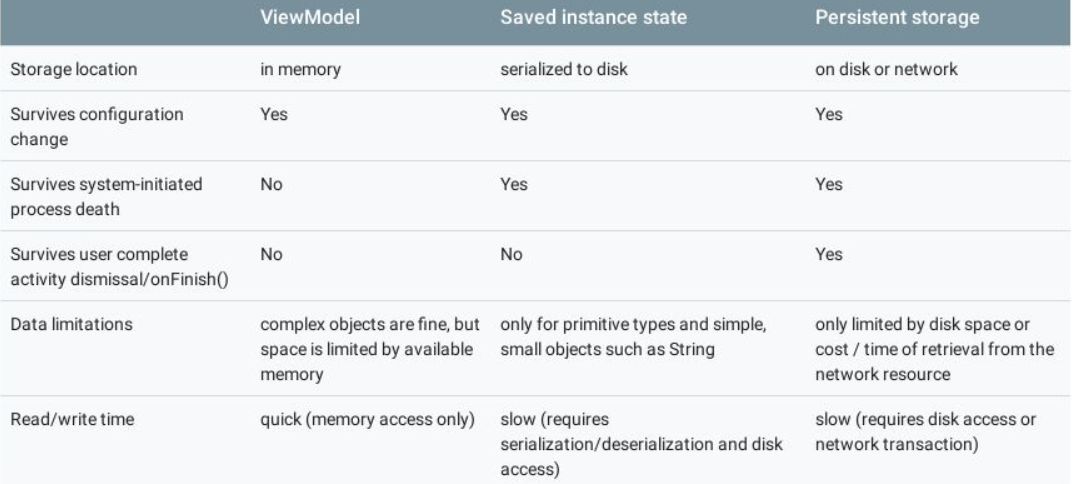
\includegraphics[scale=0.32]{persistenzarten.png}

\textbf{Observer Pattern Beispiel Counter} \\
\textit{/domain/Counter.java}
\begin{lstlisting}[language=java]
public class Counter extends Observable {
    private int value;
    public Counter(){
        value = 0;
    }
    public String getValue(){
        return Integer.toString(value);
    }
    public void incrementValue(){
        value++;
        setChanged();
        notifyObservers();
    }
    public void decrementValue(){
        value--;
        setChanged();
        notifyObservers();
    }
}
\end{lstlisting}
\textit{/presentation/MainActivity.java}
\begin{lstlisting}[language=java]
public class MainActivity extends AppCompatActivity implements Observer {
    private Counter counter;

    @Override
    protected void onCreate(Bundle savedInstanceState) {
        super.onCreate(savedInstanceState);
        setContentView(R.layout.activity_main);
        counter = new Counter();
        counter.addObserver(this);
        Button plusButton = findViewById(R.id.buttonPlus);
        Button minusButton = findViewById(R.id.buttonMinus);
        minusButton.setOnClickListener(new View.OnClickListener() {
            @Override
            public void onClick(View v) {
                counter.decrementValue();
            }
        });
        plusButton.setOnClickListener(new View.OnClickListener() {
            @Override
            public void onClick(View v) {
                counter.incrementValue();
            }
        });
    }
    @Override
    public void update(Observable o, Object arg) {
        final Counter counter = (Counter)o;
        TextView counterText = findViewById(R.id.counter);
        counterText.setText(counter.getValue());
    }
}
\end{lstlisting}

\textbf{AsyncTask und Service} \\
\textit{MainActivity.java}
\begin{lstlisting}[language=java]
public class MainActivity extends AppCompatActivity implements View.OnClickListener {
    private TextView txtMessage;
    private MessageReceiver messageReceiver;
    @Override
    protected void onCreate(Bundle savedInstanceState) {
        super.onCreate(savedInstanceState);
        setContentView(R.layout.activity_main);
        Button btnAsyncTask = findViewById(R.id.asynctaskbutton);
        Button btnService = findViewById(R.id.servicebutton);
        txtMessage = findViewById(R.id.message);
        btnAsyncTask.setOnClickListener(this);
        btnService.setOnClickListener(this);
    }
    @Override
    public void onClick(View view){
        switch(view.getId()){
            case R.id.servicebutton:
                startMessageService();
                break;
            case R.id.asynctaskbutton:
                View rootView = findViewById(android.R.id.content).getRootView();
                Task task = new Task(this, rootView);
                task.execute();
                break;
        }
    }
    @Override
    public void onResume(){
        super.onResume();
        LocalBroadcastManager lbm = LocalBroadcastManager.getInstance(getApplicationContext());
        IntentFilter intentFilter = new IntentFilter("filtermessage");
        messageReceiver = new MessageReceiver(this);
        lbm.registerReceiver(messageReceiver, intentFilter);
    }
    @Override
    public void onPause(){
        super.onPause();
        LocalBroadcastManager lbm = LocalBroadcastManager.getInstance(this);
        lbm.unregisterReceiver(messageReceiver);
    }
    public void startMessageService(){
        EditText input = findViewById(R.id.input);

        Intent intent = new Intent(this, Service.class);
        intent.putExtra("message_send", input.getText().toString());
        startService(intent);
    }
    private class MessageReceiver extends BroadcastReceiver{
        MainActivity activity;
        public MessageReceiver(MainActivity activity){
            this.activity = activity;
        }
        @Override
        public void onReceive(Context context, Intent intent) {
            String message = intent.getStringExtra("message_back");
            txtMessage.setText(message);
        }
    }
}
\end{lstlisting}
\textit{Task.java}
\begin{lstlisting}[language=java]
public class Task extends AsyncTask<String, String, String> {
    private String resp;
    ProgressDialog progressDialog;
    private Context context;
    private View view;

    public Task(Context context, View view){
        this.context = context;
        this.view = view;
    }
    @Override
    protected String doInBackground(String... strings) {
        publishProgress("Sleeping..."); // Calls onProgressUpdate()
        try {
            Thread.sleep(5000);
            resp = "Slept for 5s";

        } catch (InterruptedException e){
            e.printStackTrace();
            resp = e.getMessage();
        }
        return resp;
    }
    @Override
    protected void onPostExecute(String result){
        progressDialog.dismiss();

        TextView message = (TextView) view.findViewById(R.id.message);
        message.setText(result);
    }
    @Override
    protected void onPreExecute(){
        progressDialog = ProgressDialog.show(context,
                "ProgressDialog",
                "Wait for 5 seconds");
    }
    @Override
    protected void onProgressUpdate(String... values){ }
}
\end{lstlisting}
\textit{Service.java}
\begin{lstlisting}[language=java]
public class Service extends IntentService {
    public Service(){
        super("Service");
    }
    @Override
    protected void onHandleIntent(Intent intent) {
        String message = intent.getStringExtra("message_send");
        LocalBroadcastManager lbm = LocalBroadcastManager.getInstance(getApplicationContext());
        Intent retIntent = new Intent("filtermessage");
        retIntent.putExtra("message_back", message);
        lbm.sendBroadcast(retIntent);
    }
}
\end{lstlisting}

\textbf{Fragment Communication} \\
\textit{MainActivity.java \& GoToNextPage}
\begin{lstlisting}[language=java]
public interface GoToNextPage { void goToNextPage(); }

public class MainActivity extends AppCompatActivity implements GoToNextPage, HelloFragment.OnNameChangeListener {
    private String name;
    enum Pages {HELLO, NAME}
    private Stack<Pages> pages = new Stack<>();
    private FragmentManager fragmentManager;
    
    @Override
    protected void onCreate(Bundle savedInstanceState) {
        super.onCreate(savedInstanceState);
        setContentView(R.layout.activity_main);

        fragmentManager = getSupportFragmentManager();
        pages.push(Pages.HELLO);
        switchTo(new HelloFragment());
    }
    private void switchTo(Fragment fragment){
        Bundle args = new Bundle();
        args.putString("name", name);
        fragment.setArguments(args);
        FragmentTransaction fragmentTransaction = fragmentManager.beginTransaction();
        fragmentTransaction.replace(R.id.fragment_container, fragment);
        fragmentTransaction.addToBackStack(null);
        fragmentTransaction.commit();
    }
    public void onBackPressed(){
        if(fragmentManager.getBackStackEntryCount() <= 1){
            finish();
        } else {
            pages.pop();
            fragmentManager.popBackStack();
        }
    }
    @Override
    public void goToNextPage() {
        switch (pages.peek()) {
            case HELLO:
                pages.push(Pages.NAME);
                switchTo(new NameFragment());
                break;
            case NAME:
                pages.clear();
                pages.push(Pages.HELLO);
                switchTo(new HelloFragment());
                break;
        }
    }
    @Override
    public void onNameChanged(String name) {
        this.name = name;
    }
}
\end{lstlisting}
\textit{HelloFragment.java}
\begin{lstlisting}[language=java]
public class HelloFragment extends Fragment {

    private GoToNextPage activity;

    public interface OnNameChangeListener {
        void onNameChanged(String name);
    }
    @Override
    public View onCreateView(LayoutInflater inflater, ViewGroup container, Bundle savedInstanceState) {
        View root = inflater.inflate(R.layout.fragment_hello, container, false);
        root.findViewById(R.id.enter).setOnClickListener(v -> activity.goToNextPage());
        EditText name = root.findViewById(R.id.nameInput);
        name.addTextChangedListener(new TextWatcher() {
            @Override
            public void beforeTextChanged(CharSequence s, int start, int count, int after) { }

            @Override
            public void onTextChanged(CharSequence s, int start, int before, int count) {
                ((OnNameChangeListener) getActivity()).onNameChanged(s.toString());
            }
            @Override
            public void afterTextChanged(Editable s) { }
        });
        return root;
    }
    @Override
    public void onAttach(Context activity) {
        super.onAttach(activity);
        if (activity instanceof GoToNextPage) {
            this.activity = (GoToNextPage) activity;
        } else {
            throw new AssertionError("Activity must implement GoToNextPage!");
        }
        if (!(activity instanceof OnNameChangeListener)) {
            throw new AssertionError("Activity must implement OnNameChangeListener!");
        }
    }
}
\end{lstlisting}
\textit{NameFragment.java}
\begin{lstlisting}[language=java]
public class NameFragment extends Fragment {

    @Override
    public View onCreateView(LayoutInflater inflater, ViewGroup container, Bundle savedInstanceState) {
        View root = inflater.inflate(R.layout.fragment_name, container, false);
        String data = getArguments().getString("name");
        TextView nameLabel = root.findViewById(R.id.nameLabel);
        nameLabel.setText("Willkommen" + data);
        return root;
    }
    @Override
    public void onAttach(Context activity) {
        super.onAttach(activity);
        if (!(activity instanceof GoToNextPage)) {
            throw new AssertionError("Activity must implement GoToNextPage!");
        } } }
\end{lstlisting}
\end{multicols*}
\end{document}
